\usetikzlibrary{patterns}
\usetikzlibrary{decorations.pathmorphing}
\usepackage{titlesec,calc}
% \renewcommand{\familydefault}{\sfdefault}

\titleformat{\section}[hang]
{\normalfont\bfseries}
{\thesection.}{0.5em}{}
 \titlespacing{\section}{0pt}{3pt}{0pt} % Horizontal space, before space, after space

\mode<presentation>
{
  \usetheme{CambridgeUS}
  \usecolortheme{whale}
  \usecolortheme{lily}

  \setbeamercovered{transparent}
  \usefonttheme[onlymath]{serif}
}

\title[Pendulum Balancing] % (optional, use only with long paper titles)
{\large \course: \coursename \\[5pt] \semesteryear\\[5pt] Balancing a Pendulum}

\subtitle
{} % (optional)

\author[\instructorshort]% (optional, use only with lots of authors)
{\instructorlong\credits}
%{T. Vincent\inst{1} \and S.~Another\inst{2}}
% - Use the \inst{?} command only if the authors have different
%   affiliation.

\institute[\instituteshort] % (optional, but mostly needed)
{\institutelong}


\date % (optional)
{}



% If you have a file called "university-logo-filename.xxx", where xxx
% is a graphic format that can be processed by latex or pdflatex,
% resp., then you can add a logo as follows:

%\pgfdeclareimage[height=1.1cm]{university-logo}{UniversityLogo}
%\logo{\pgfuseimage{university-logo}}



% Delete this, if you do not want the table of contents to pop up at
% the beginning of each subsection:
%\AtBeginSection[]
%{
%  \begin{frame}<beamer>{Outline}
%    \tableofcontents[currentsection,currentsubsection]
%  \end{frame}
%}


% If you wish to uncover everything in a step-wise fashion, uncomment
% the following command:

%\beamerdefaultoverlayspecification{<+->}



\begin{document}
\maketitle
 
In the last document, we discussed a model for a balancing robot. 

\begin{figure}[h]
\begin{center}
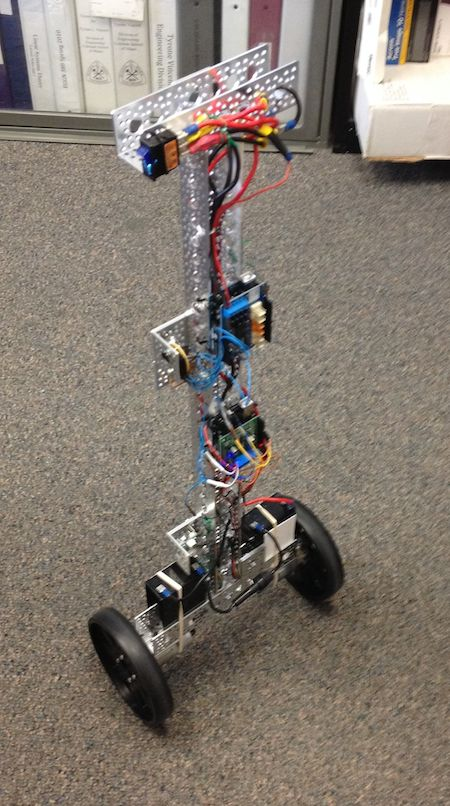
\includegraphics[height=2.5in]{Graphics/robot}\hspace{1in}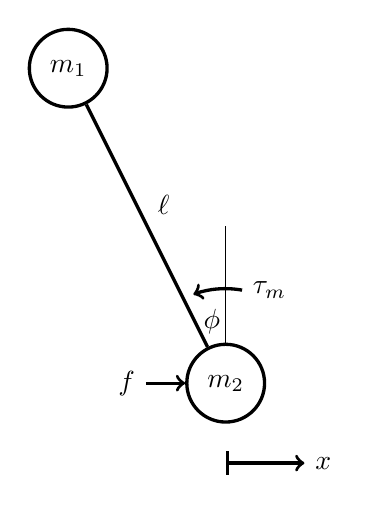
\begin{tikzpicture}[very thick,
sysblock/.style={draw,rectangle,inner sep=6pt,minimum width=1.5cm,minimum height=1.2cm,very thick},
delayblock/.style={draw,rectangle,inner sep=6pt,minimum width=0.5cm,minimum height=1.0cm,very thick},
node/.style={fill,inner sep=0pt,outer sep=0pt},
summer/.style={circle,draw,very thick,inner sep=5pt}]

\draw (0,0) node[summer] (M1) {$m_{1}$};
\draw (2,-4) node[summer] (M2) {$m_{2}$};

\draw  (M1) -- node[pos=.5, above right] {$\ell$} (M2);
\draw[thin]  (M2) -- ++(0,2);
\draw (M2.110) node[above] {$\phi$};
\draw[->] (M2) ++(80:1.2) node[right] {$\tau_{m}$} arc (80:110:1.2);
\draw[|->] (M2.-90) ++(0,-.5) -- ++(1,0) node[right] {$x$};
%\draw[|->] (M1.90) ++(0,.5) -- ++(1,0) node[right] {$x_{2}$};
%\draw[|->] (M1.180) ++(-.5,0) -- ++(0,1) node[above] {$y_{2}$};
\draw[->] (M2.180) ++(-.5,0) node[left] {$f$} -- (M2.180);

\end{tikzpicture}
\end{center}
\caption{Idealized component diagram for pendulum robot}
\end{figure}

\begin{equation}\label{eqn:model}
\begin{aligned}
\ddot{\phi}&= \frac{(g(m_{1}+m_{2})-m_{1}\ell\cos\phi(\dot{\phi})^2) \sin\phi -  \cos{\phi}b_{x}\dot{x}   -  \frac{(m_{1}+m_{2})}{m_{1}\ell}b_{\phi}\dot{\phi}  + \left( \frac{(m_{1}+m_{2})}{m_{1}\ell}+ \frac{\cos{\phi}}{r}\right)\tau_{m}}{\ell\left(m_{2} +m_{1}\sin^{2}\phi\right)} \\
\ddot{x} &= \frac{gm_{1}\cos\phi\sin\phi - m_{1}\ell\sin\phi(\dot{\phi})^2 -b_{x}\dot{x} - \frac{\cos\phi}{\ell}b_{\phi}\dot{\phi} +\left( \frac{\cos\phi}{\ell} + \frac{1}{r} \right)\tau_{m}}{(m_{2} + m_{1}\sin^2\phi)}
\end{aligned}
\end{equation}
At this point, you should have done experiments to find the parameters for your robot.


We wish to design a control system that will stabilize the pendulum around $\phi=0$. The nonlinear model is fairly complex to use for design. However, since the point of the control system is to regulate the system to stay near a specific operating point, we can use linear approximations (i.e. first order Taylor series) of the sine and cosine functions around this point. For $\phi\approx 0$ and $\dot{\phi}\approx 0$ this is $\sin(\phi)\approx\phi$, $\sin^2(\phi)\approx 0$ and $\cos(\phi)\approx 1$. In order to keep the model simple, we will also assume that the damping terms $b_{x}$ and $b_{\phi}$ are small enough to be set to zero. (They can actually easily be added, but the resulting controller won't change that much, and it will make things a little simpler for you. Note that we will always go back an verify that the controller works using the full, nonlinear system model)  This gives the linearized dynamics
\begin{align*}
\ddot{\phi} &= a \phi + c \tau_{m} \\
\ddot{x} &=  b\phi + d \tau_{m} 
\end{align*}
where
\begin{align*}
a &= \frac{g(m_{1}+m_{2})}{\ell m_{2}}\\
c & = \frac{1}{\ell m_{2}}\left( \frac{(m_{1}+m_{2})}{m_{1}\ell}+ \frac{1}{r}\right) \\
b &= \frac{m_{1}}{\ell m_{2}}\\
d & = \frac{1}{m_{2}}\left( \frac{1}{\ell}+ \frac{1}{r}\right)
\end{align*}

Taking the Laplace Transforms of both sides,
\begin{align*}
s^2\phi(s) &=  a \phi(s) + c\tau_{m}(s)\\
s^{2}X(s) &= b\phi(s) + d\tau_{m}(s)
\end{align*}
We can solve these equations for the two transfer functions $\frac{\phi(s)}{\tau_{m}(s)}$ and $\frac{X(s)}{\tau_{m}(s)}$. This can easily done with $b\neq 0$, but for our robots, since we will be controlling the robot to be upright, it will turn out that the term $b\phi(s)$ will be small. Thus, we take the following as the transfer functions. (If you use Matlab, it isn't really a big deal to keep $b\neq 0$, and you can try the design both ways to see what effect there is)
\begin{align*}
\frac{\phi(s)}{\tau_{m}(s)} & = \frac{c}{s^{2} -a} \\
\frac{X(s)}{\tau_{m}(s)} & =\frac{d}{s^{2}}
\end{align*}
Only one problem: we can't directly measure $\phi$ with a gyroscope, we can only measure $\dot{\phi}$. However, consider the following trick: instead of stabilizing $\phi$ at 0, what if we try and stabilize $\dot{\phi}$ at 0? Generally, controlling $\dot{\phi}=0$ would ensure $\phi$ is a constant, but we would not necessarily know what that constant is. However, for this system, because of gravity there is no way that we can achieve $\dot{\phi}=0$ {\em without} being at one of the equilibrium points of $\phi=0$ or $\phi=\pi$.  To consider $\dot{\phi}$ as the output of the system,  we will multiply our transfer function by $s$:
\[
\frac{\dot{\phi}(s)}{\tau(s)} = \frac{cs}{s^{2} -a}.
\]
We can also scale $x$ by $r$ to recover the wheel rotation $\theta$
\[
\frac{\theta(s)}{\tau(s)} = \frac{d/r}{s^{2}}.
\]


We now have two different models that we can use. One is the more accurate, nonlinear, model given by the Simulink subsystem
\begin{center}
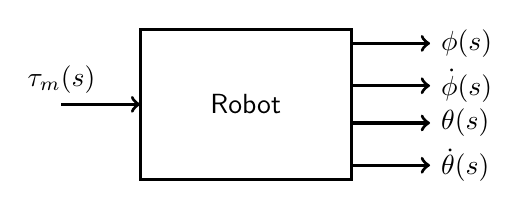
\begin{tikzpicture}[inner sep=0pt,outer sep=0pt,very thick,
sysblock/.style={draw,rectangle,inner sep=2pt,minimum width=1.5cm,minimum height=1.25cm,very thick}]

\draw (0,0) node[sysblock,minimum height=.75in] (a) {\begin{minipage}{1in}\centering\textsf{Robot}\end{minipage}};

\draw[<-] (a.180) -- ++(-1,0) node[above=4pt] {$\tau_{m}(s)$};
\draw[->] (a.30) -- ++(1,0) node[right=4pt] {$\phi(s)$};
\draw[->] (a.10) -- ++(1,0) node[right=4pt] {$\dot{\phi}(s)$};
\draw[->] (a.-10) -- ++(1,0) node[right=4pt] {$\theta(s)$};
\draw[->] (a.-30) -- ++(1,0) node[right=4pt] {$\dot{\theta}(s)$};
\end{tikzpicture}
\end{center}
The other is an approximate, linear model that only keeps track of $\dot{\phi}$ and $\theta(s)$ 

\begin{center}
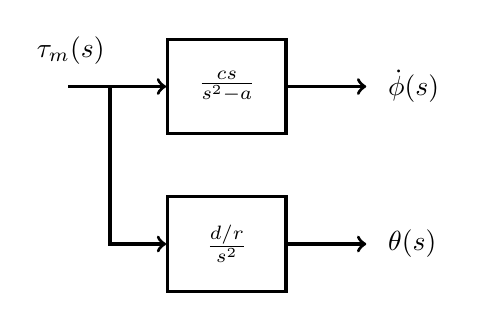
\begin{tikzpicture}[very thick,
sysblock/.style={draw,rectangle,inner sep=6pt,minimum width=1.5cm,minimum height=1.2cm,very thick},
delayblock/.style={draw,rectangle,inner sep=6pt,minimum width=0.5cm,minimum height=1.0cm,very thick},
node/.style={fill,inner sep=0pt,outer sep=0pt},
summer/.style={circle,draw,very thick,inner sep=5pt}]

\draw (-2,0) node[node] (c) {};
\draw (0,0) node[sysblock] (a) {$\frac{cs}{s^{2}-a}$};
\draw (0,-2) node[sysblock] (b) {$\frac{d/r}{s^{2}}$};

\draw[->] (c.0) node[above=4pt] {$\tau_{m}(s)$} -- (a.180);
\draw[->] (c.0)  -- ++(0.5,0) |- (b.180);
\draw[->] (a.0) -- ++(1,0) node[right=4pt] {$\dot{\phi}(s)$};
\draw[->] (b.0) -- ++(1,0) node[right=4pt] {$\theta(s)$};
\end{tikzpicture}
\end{center}
This linear model can be used if the following hold:
\begin{itemize}
\item  $\phi$ is small
\item  $\dot{\phi}$ is small
\item the damping terms are negligible.
\end{itemize}

You can use the simpler model for designing the feedback control system. First, let's add the other components to the robot, starting with the motor. In the following block diagram, we have (again, for simplicity) assumed the motor inductance $L_{a}=0$. The motor voltage is $V_{a}(s)$.

\begin{center}
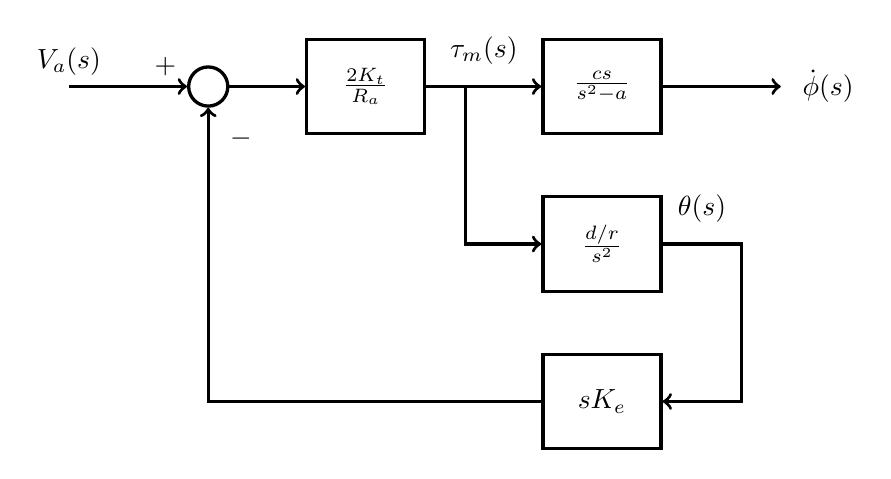
\begin{tikzpicture}[very thick,
sysblock/.style={draw,rectangle,inner sep=6pt,minimum width=1.5cm,minimum height=1.2cm,very thick},
delayblock/.style={draw,rectangle,inner sep=6pt,minimum width=0.5cm,minimum height=1.0cm,very thick},
node/.style={fill,inner sep=0pt,outer sep=0pt},
summer/.style={circle,draw,very thick,inner sep=5pt}]

\draw (-5,0) node[summer] (sum) {};
\draw (-3,0) node[sysblock] (K) {$\frac{2K_{t}}{R_{a}}$};
\draw (0,0) node[sysblock] (a) {$\frac{cs}{s^{2}-a}$};
\draw (0,-2) node[sysblock] (b) {$\frac{d/r}{s^{2}}$};
\draw (0,-4) node[sysblock] (c) {$sK_{e}$};

\draw[->] (K.0)  -- node[above=4pt] {$\tau_{m}(s)$} (a.180);
\draw[->] (K.0)  -- ++(0.5,0) |- (b.180);
\draw[->] (a.0) -- ++(1.5,0) node[right=4pt] {$\dot{\phi}(s)$};
\draw[->] (b.0) -- node[above=4pt] {$\theta(s)$} ++(1,0) |- (c.0);
\draw[->] (c.180) -| (sum.-90) node[below right=4pt] {$-$};
\draw[->] (sum.0) -- (K);
\draw[<-] (sum.180) node[above left] {$+$} -- ++(-1.5,0) node[above] {$V_{a}(s)$};
\end{tikzpicture}
\end{center}
Simplifying the block diagram, we get the following transfer function with motor voltage as the input:
\begin{align*}
\frac{\dot{\phi}(s)}{V_{a}(s)} &= \frac{\frac{2K_{t}}{R_{a}}}{1+\frac{2K_{t}K_{e}d}{R_{a}rs}}\frac{cs}{s^{2}-a}\\
& =  \frac{es^2}{(s+f)(s^{2}-a)}
\end{align*}
where
\begin{align*}
e & = \frac{2K_{t}c}{R_{a}} \\
f & = \frac{2K_{t}K_{e}d}{R_{a}r}
\end{align*}

In the next section, we will investigate the design of a controller $C(s)$ that operates within the following unity-gain feedback control system to stabilize $\dot{\phi}$. 

\begin{center}
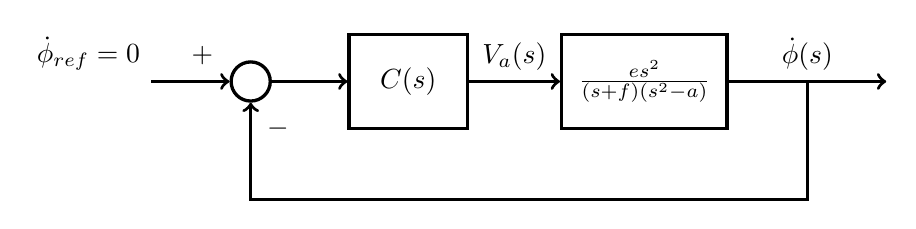
\begin{tikzpicture}[very thick,
sysblock/.style={draw,rectangle,inner sep=6pt,minimum width=1.5cm,minimum height=1.2cm,very thick},
delayblock/.style={draw,rectangle,inner sep=6pt,minimum width=0.5cm,minimum height=1.0cm,very thick},
node/.style={fill,inner sep=0pt,outer sep=0pt},
summer/.style={circle,draw,very thick,inner sep=5pt}]

\draw (0,0) node[summer] (sum) {};
\draw (2,0) node[sysblock] (C) {$C(s)$};
\draw (5,0) node[sysblock] (G) {$\frac{es^2}{(s+f)(s^{2}-a)}$};

\draw[<-] (sum.180) node[above left=2pt] {$+$} -- ++(-1,0) node[above left] {$\dot{\phi}_{ref}=0$};
\draw[->] (sum.0) -- (C.180);
\draw[->] (C.0) --  node[pos=.5,above]  {$V_{a}(s)$} (G.180);
\draw[->] (G.0) -- node[above] {$\dot{\phi}(s)$} ++(2,0);
\draw[->] (G.0) ++(1,0) -- ++(0,-1.5) -| (sum.-90) node[below right=2pt] {$-$};
\end{tikzpicture}
\end{center}


\section{Pendulum Control}

The controller that we will design, $C(s)$, will provide voltage command, $v_{a}$, which is calculated based on measurements of the angular velocity $\dot{\phi}$, compared to the desired reference, $0$ rad/s. Since the system under control is unstable, the control design is somewhat different than the standard methods in EENG307. However, we can use the root locus to help us with our design. 


\begin{itemize}
\item Calculate the parameters $c$, $f$ and $a$ for your robot.
\item Check that proportional control will not work by plotting the root locus of $\frac{es^2}{(s+f)(s^{2}-a)}$. Verify that there is an unstable closed loop pole for any value of $K$ when $C(s)=K$.
\item Now, try a controller of the form
\[
C(s) = K\frac{(s+\alpha)(s+\beta)}{(s+\gamma)(s-\delta)}
\]
Where $\alpha, \beta$, $\gamma$ and $\delta$ are positive constants to be found. Note that the term $(s-\delta)$ is not a typo - we are going to include an unstable pole with this controller. 
%In order to keep the DC gain of the controller positive ($C(0)$) we also include a negative gain $-K$. 
Choose $\alpha=\sqrt{a}$, $\beta \approx 1$, $\gamma$ a small value, and $\delta$ a little smaller than $\sqrt{a}$, and plot the root locus of $\frac{(s+\alpha)(s+\beta)}{(s+\gamma)(s-\delta)}\frac{es^2}{(s+f)(s^{2}-a)}$ (don't forget the negative sign out front). Vary the values of $\alpha$, $\beta$, $\gamma$, and $\delta$ to see the effect of each. You will probably need to zoom in to the origin on your root locus to see the interesting part of the plot. %You may want to use \texttt{sisotool} to help you do this, with a warning - when you add an unstable pole, \texttt{sisotool} will include a term of the form $(-s/\delta + 1)$, so you will have to go to the \textsf{Control and Estimation Tools Manager}, click on the \textsf{Compensator Editor} tab, and multiply the gain in the \textsf{Compensator} block by -1 to get back to the form above.
\item From the root locus, choose a value of $K$ so that the closed loop poles will be well damped. Plot the impulse response (this is what you would see if the pendulum was bumped). You may want to re-adjust $K$, and/or $\alpha$, $\beta$, $\gamma$ or $\delta$ depending on what you see in the impulse response.
\item Using Simulink, simulate the closed loop behavior with your controller applied to the nonlinear model. Some discussion of this is in the next section. 
\end{itemize}

\section{Signs and scaling}

When implementing your controller, you will need to be careful about the signs of the actuator and sensor signals, and the scaling associated with them. For the design above, we have assumed that for a positive motor current, the clockwise torque will act on the wheels, creating a counter clockwise torque on the pendulum. Also, we have assumed that the motion $\dot{\phi}$ is measured with counter-clockwise motion as positive. Depending on how you mounted and configured your motors and gyro, this convention may or may not hold. You will want to verify that a positive motor voltage will tend to cause a positive angular velocity. If not, change the sign of either the gyro or the motor voltage (but not both!)

Another thing to watch out for is the required scaling in order to implement your controller. Note that the controller designed above outputs a signal in units of Volts and has an input with units of rad/s. However, in the Arduino, you will create a output voltage (or really, PWM signals) by choosing a specific integer, and likewise the gyro reading will be an integer representing some voltage and will definitely not have units of rad/s. Make sure you do the right conversions.

\section{Control implementation on a micro-controller}

When implementing the PID controller we used the discrete approximation for the integral and derivative. The derivative approximation was
\[
e(t) = \frac{dy(t)}{dt} \approx \frac{y(t) - y(t-T_{s})}{T_{s}}, 
\]
where $T_{s}$ is the sample time.  Using discrete time signal notation this becomes
\[
e[k]  = \frac{y[k] - y[k-1]}{T_{s}},
\]
and solving for $y[k]$ gives us
\[
y[k] = y[k-1] + T_{s}e[k].
\]
We can use this same derivative approximation to convert an arbitrary first order differential  equation to a recursive equation. For example, if we have a desired controller of the form
\[
\frac{Y(s)}{E(s)} = K\frac{as+1}{bs+1}
\]
where $a$ and $b$ are constants, then
\begin{align*}
(bs+1)Y(s) &= K(as+1)E(s),\\
bsY(s) + 1Y(s) &= KasE(s) + KE(s), 
\end{align*}
and finding the inverse Laplace transform gives us
\begin{align*}
b\frac{d}{dt}y(t) + y(t) & = Ka\frac{d}{dt}e(t) + K e(t).
\end{align*}
Using the approximation $\frac{dy(t)}{dt} \approx \frac{y(t) - y(t-T_{s})}{T_{s}}$ and $\frac{de(t)}{dt} \approx \frac{e(t) - e(t-T_{s})}{T_{s}}$, and converting to discrete time signals results in
\[
b\frac{y[k] - y[k-1]}{T_{s}} + y[k] = Ka\frac{e[k] - e[k-1]}{T_{s}} + Ke[k].
\]
We can solve this equation for $y[k]$ to give our final recursive formula 
\[
y[k] = \frac{1}{b+T_{s}}\left(b y[k-1]  + K(a+T_{s})e[k] - Kae[k-1]\right).
\]

This can be extended to higher order transfer functions by introducing intermediate variables. For example, suppose we have the controller
\[
C(s) = \frac{U(s)}{E(s)} = K\frac{(as+1)(cs+1)}{(bs+1)(ds+1)}
\]
We want to calculate the signal $u$, based on measurements of $e$. We can introduce the intermediate variable $v$, defined via 
\[
\frac{V(s)}{E(s)} = K\frac{(as+1)}{(bs+1)}.
\]
Then we have
\[
\frac{U(s)}{V(s)} = \frac{(cs+1)}{(ds+1)}.
\]
The controller can be implemented by calculating $v$ from $e$, and then calculating $u$ from $v$.

\section{Anti-windup for unstable terms}

For the integral term in the PID control, we implemented an anti-windup scheme that re-calculated the integral term when actuator saturation occured. Anti-windup is necessary for any unstable term in a controller, for example if either $b<0$ or $d<0$. It is most convenient if the unstable term is the last one, so let's suppose that $d<0$. The recursive formula would be
\[
u[k] = \frac{1}{d+T_{s}}\left(d u[k-1]  + K(c+T_{s})v[k] - Kcv[k-1]\right).
\]
Suppose the actuator is saturated when $|u| = u_{max}$. In this case, if we find that $u$ calculated using the controller had magnitude greater than $u_{max}$, we set it so that its magnitude is exactly $u_{max}$. The code would look something like this:

\texttt{\\
\vdots\\
u = (1/(d+Ts))*(d*u\_past + K*(c+Ts)*v - K*c*v\_past); \\
if (abs(u)>umax) \{ u=sgn(u)*umax; \}\\
u\_past = u;\\
v\_past = v;\\
\vdots\\
}
where \texttt{sgn} is the signum function that returns 1 if the argument is positive and -1 if it is negative. This is not a native function for the Arduino, but is easily implemented.

\section{Further Hierarchical Control Loops}

The controller designed above can be applied to the nonlinear model. 
\begin{center}
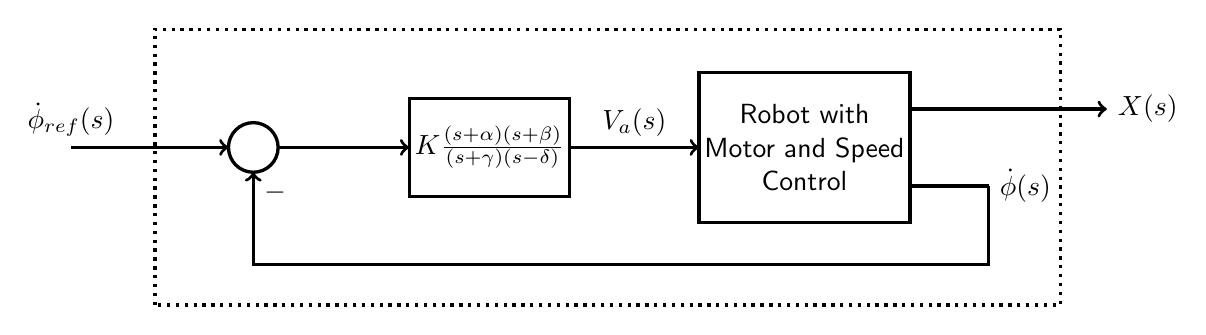
\begin{tikzpicture}[inner sep=0pt,outer sep=0pt,very thick,
sysblock/.style={draw,rectangle,inner sep=2pt,minimum width=1.5cm,minimum height=1.25cm,very thick}]
\draw (-7,0) node[draw,circle] (sum) {$\rule{0pt}{18pt}$};
\draw (-4,0) node[sysblock] (c) {$K\frac{(s+\alpha)(s+\beta)}{(s+\gamma)(s-\delta)}$};
\draw (0,0) node[sysblock,minimum height=.75in] (a) {\begin{minipage}{1in}\centering\textsf{Robot with Motor and Speed Control}\end{minipage}};
\draw[<-] (sum.180) -- ++(-2,0) node[above=4pt] {$\dot{\phi}_{ref}(s)$};
\draw[->] (sum.0) -- (c.180);
\draw[->] (c.0) -- node[above=4pt] {$V_{a}(s)$} (a.180);
\draw[->] (a.20) -- ++(2.5,0) node[right=4pt] {$X(s)$};
\draw[-] (a.-20) -- ++(1,0) node[right=4pt] {$\dot{\phi}(s)$};
\draw[->] (a.-20) ++(1,0) -- ++(0,-1) -| (sum.-90) node[below right=4pt] {$-$};
\draw[dotted] (-8.25,-2) rectangle (3.25,1.5);
\end{tikzpicture}
\end{center}

Via simulation, you will find that with $\dot{\phi}_{ref}=0$, this controller will successfully balance the robot, in that $\dot{\phi}=0$ and $\phi$ will also be close to 0, even if the initial condition $\phi(0) \neq 0$.  However, you will also find that the controller will cause $x$ to vary quite a bit. In order to have a functional robot, we need to also control the horizontal position. However,  now we have yet another level of encapsulation:

\begin{center}
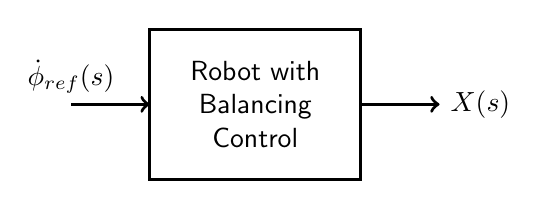
\begin{tikzpicture}[inner sep=0pt,outer sep=0pt,very thick,
sysblock/.style={draw,rectangle,inner sep=2pt,minimum width=1.5cm,minimum height=1.25cm,very thick}]

\draw (0,0) node[sysblock,minimum height=.75in] (a) {\begin{minipage}{1in}\centering\textsf{Robot with Balancing Control}\end{minipage}};

\draw[<-] (a.180) -- ++(-1,0) node[above=4pt] {$\dot{\phi}_{ref}(s)$};
\draw[->] (a.0) -- ++(1,0) node[right=4pt] {$X(s)$};
\end{tikzpicture}
\end{center}

Can you design a controller that will regulate $x$ around a desired value, using $\dot{\phi}$ as an actuator?


\end{document}  
